%NYU 2019 Grad Computational Physics Homework 3

\documentclass[12pt, graphicx]{article}
\pagestyle{plain}
\baselineskip 18pt
\textwidth 6.5in
\textheight 7.8in
\oddsidemargin 0.1in
\evensidemargin 0.1in
\topmargin 0.3in
\parindent 0pt
\linespread{1.5}
\setlength{\parskip}{2.5mm}

\usepackage{graphicx, psfrag, epsfig}
\usepackage[font = small, format = plain, labelfont = bf, textfont = it, justification = raggedright, singlelinecheck = false]{caption}
\usepackage{subfig}
\usepackage{amsmath, amssymb}
\usepackage{geometry}
%\usepackage[symbol]{footmisc}

\renewcommand\tablename{Table}
\renewcommand\figurename{Fig.}
\renewcommand{\thefootnote}{\fnsymbol{footnote}}


\begin{document}
\title{Computational Physics Homework 3}
\author{Hao Li\footnotemark[2]}
\footnotetext[2]{hl3270@nyu.edu~~UID:N12137527}
\date{\today}


\maketitle

\section*{Problem 1}
\subsection*{a)}
The plot of the number of sunspots as a function of time from \textquotedblleft sunspots.txt\textquotedblright is shown in Figure. \ref{fig:sunspots}. From the graph, we can see 24~25 evenly distributed small peaks in the whole 3143 months. So the length of the cycle in months should be 
\begin{equation}
\frac{3143}{25}\approx125.7<T/\mathrm{mo}<\frac{3143}{24}\approx131.0
\end{equation}
In years, then the period is approximately 
\begin{equation}
10.5\mathrm{yr}<T<10.9\mathrm{yr}
\end{equation}
which agrees with the common sense that the period of sunspots are around 11 years. 

\begin{figure}[ht]
\centering
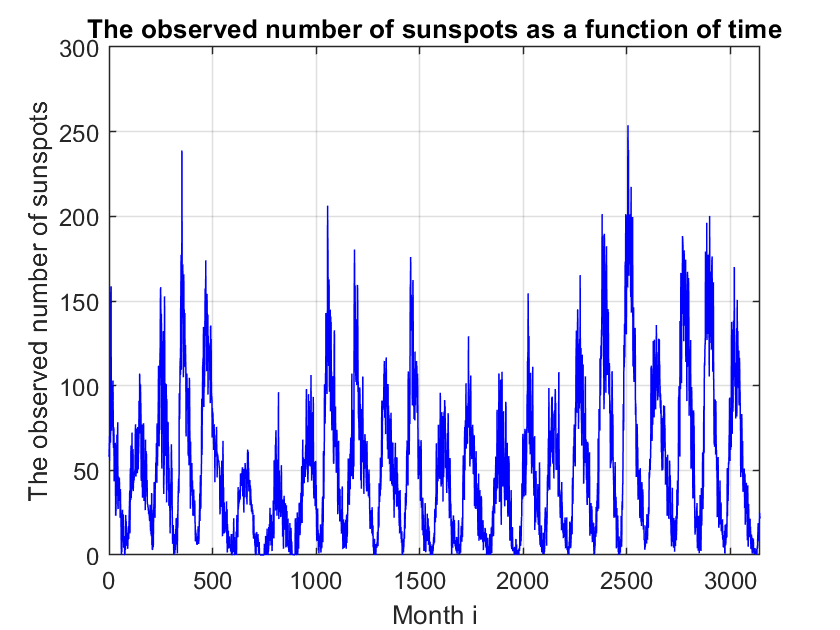
\includegraphics[width = 120mm]{sunspots.png}
\caption{The number of sunspots as a function of time from \textquotedblleft sunspots.txt\textquotedblright. }
\label{fig:sunspots}
\end{figure}

\subsection*{b)}
For $N$ evenly distributed one dimensional data points $y_n$, the conventional discrete Fourier transform (DFT) is defined as
\begin{equation}
c_k=\displaystyle\sum_{n=0}^{N-1}y_n\mathrm{exp}\left(-\mathrm{i}\frac{2\pi kn}{N}\right)
\label{eq:dft}
\end{equation}
$c_{N-r}=c_r^*$, where $^*$ is the complex conjugate. So the interval $k\in[0, \frac{N}{2}$ is enough to get all the information. \par
The code to calculate the discrete Fourier transform is available in \textquotedblleft fourier\_transform.h\textquotedblright, attached in the folder. By inputing an array of evenly distributed position of data, the code gives out the real part and imaginary parts of coefficients of DFT in Eq. \ref{eq:dft}.\par
It is shown in Figure. \ref{fig:dft} the magnitude squared of theFourier coefficients, power spectrum of the sunspot signal.
\begin{equation}
|c_k|^2=\displaystyle\sum_{n=0}^{N-1}y_n\mathrm{exp}\left(-\mathrm{i}\frac{2\pi kn}{N}\right)=\left(\displaystyle\sum_{n=0}^{N-1}y_n\cos\left(\frac{2\pi kn}{N}\right)\right)^2+\left(\displaystyle\sum_{n=0}^{N-1}y_n\sin\left(\frac{2\pi kn}{N}\right)\right)^2
\end{equation}

\begin{figure}[ht]
\centering
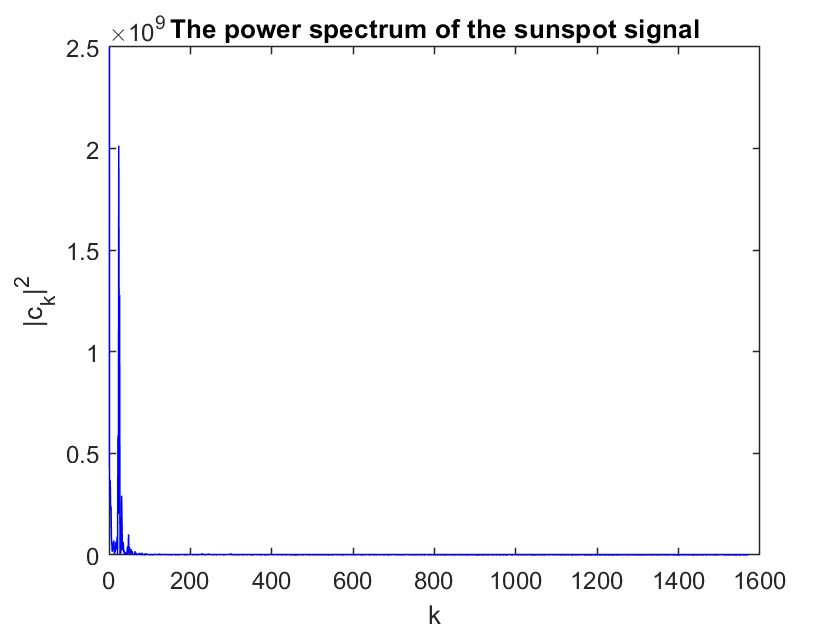
\includegraphics[width = 120mm]{powerspectrum.png}
\caption{The power spectrum of the sunspot signal from \textquotedblleft sunspots.txt\textquotedblright. }
\label{fig:dft}
\end{figure}

It is clear that there is a sharp peak within $k\in[0,60]$, so now a more detailed plot within this range is as shown in Figure. \ref{fig:dftdetail}. In this plot, we can see there is a noticable peak at about 
\begin{equation}
k\approx24,25
\end{equation}
Also the high frequency noise of the sunspot data is really small compared with this peak. What's more, there is also a small peak near $k=0$. In Figure. \ref{fig:sunspots}, we can see that the maximum amplitude if each small peak has a larger period, where we can see valleys at $k\approx750,1750$, i.e. there is about three larger period of the data, which means there should be a small peak at $k\approx3$. This agrees with the power spectrum in Figure. \ref{fig:dftdetail}.

\begin{figure}[ht]
\centering
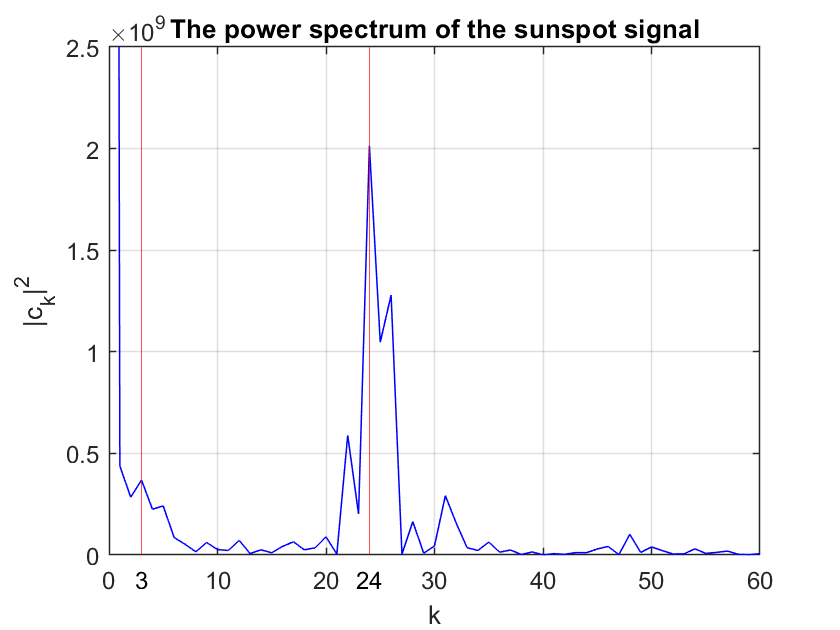
\includegraphics[width = 120mm]{powerspectrum_detailed.png}
\caption{The power spectrum of the sunspot signal from \textquotedblleft sunspots.txt\textquotedblright, within $k\in[0,60]$. There is a noticable peak at about $k\approx24,25$, which agrees with there are about 24 to 25 periods in the entire data range. Also, there is a small peak at $k\approx3$, which maches with a weaker oscillation of larger period, including about three periods in the entire time interval.}
\label{fig:dftdetail}
\end{figure}

Since the number of sunspots are always positive, $c_0$ for the sunspot signal is extremly large compared with other coefficients. But the meaning for this coefficient is just the sum (average if in $\gamma_k=\frac{c_k}{N}$ notation) of the data ($T\to\infty$), which has nothing to do with finite period of the signal, so we just ignore it.

\subsection*{c)}
Just as given in b), the approximate value of $k$, to which the peak in Figure. \ref{fig:dftdetail} correspond, is about 24 or 25. Refer to Fihure. \ref{fig:sunspots}, the left boundary $k=0$ correspond to a peak, while the right boundary $k=3142$ is near a valley. So we can reasonably approximate the entire 3143 months contains 24.5 periods. that is 
\begin{equation}
k\approx24.5
\end{equation}
The period of the sine wave with his value of $k$: $\sin\left(\frac{2\pi kt}{N}\right)$, is
\begin{equation}
T=\frac{2\pi}{\omega}=\frac{2\pi N}{2\pi k}=\frac{N}{k}\approx\frac{3143}{24.5}\mathrm{mo}\approx128.9\mathrm{mo}\approx10.7\mathrm{yr}
\end{equation}
which matches with the period derived in a), and with the knowledge that the period of sunspots is about 11 years. 

\section*{Problem 2}
\subsection*{a)}
With the convenience of showing the image and the requirement of the problem to use some prepackaged functions in part c), here we use python instead of C to deal with this problem. The program to plot the blurred photo, as well as later in part b) and c) the point spread function and the unblurred photo, is available in \textquotedblleft Hw\_3-2.ipynb\textquotedblright. The data in \textquotedblleft blur.txt\textquotedblright is a $1024\times1024$ two-dimensional array, the density plot of which is shown in Figure. \ref{fig:blur}. 

\begin{figure}[ht]
\centering
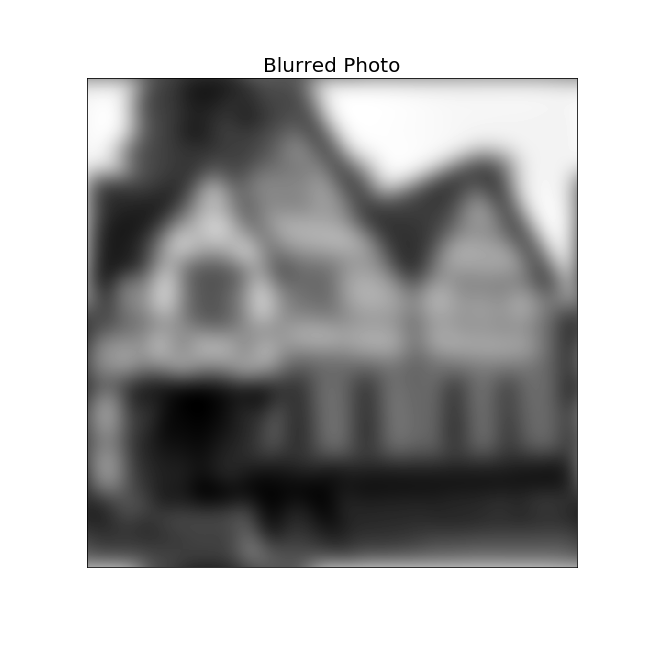
\includegraphics[width = 100mm]{blurred.png}
\caption{The blurred photo of \textquotedblleft blur.txt\textquotedblright.}
\label{fig:blur}
\end{figure}

\subsection*{b)}
Since the point spread function in this problem is given as the Gaussian
\begin{equation}
f(x,y)=\mathrm{exp}\left(-\frac{x^2+y^2}{2\sigma^2}\right),\sigma=25
\label{eq:psf}
\end{equation}
The density plot of the Gaussian point spread function Eq. \ref{eq:psf} centered at the vertices of the plot, is given in Figure. \ref{fig:psf}. We can clearly see four small bright patches in corners of the image. 

\begin{figure}[ht]
\centering
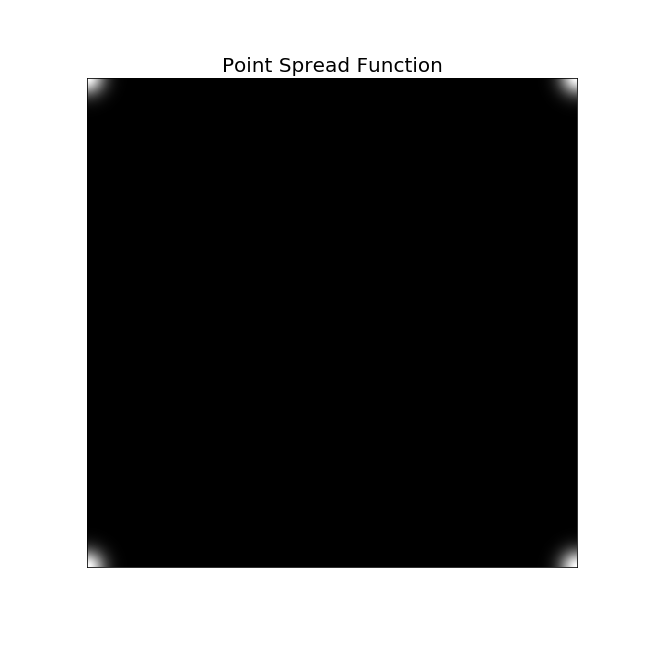
\includegraphics[width = 100mm]{point_spread.png}
\caption{The density plot of the point spread function $f(x,y)=\mathrm{exp}\left(-\frac{x^2+y^2}{2\sigma^2}\right),\sigma=25$.}
\label{fig:psf}
\end{figure}

\subsection*{c)}
Given the the blurred photo $b(x,y)$ and the point spread function $f(x,y)=\mathrm{exp}\left(-\frac{x^2+y^2}{50}\right)$, and the dimension of the photo $L=1024$, to get the unblurred photo, first Fourier transform the two function into $\tilde{b}_k$ and $\tilde{f}_k$, then divide them 
\begin{equation}
\tilde{a}_k=\frac{\tilde{b}_k}{L^2\tilde{f}_k}
\end{equation}
Next, inverse Fourier transform $\tilde{a}_k$ into $a(x,y)$, then the matrix $a(x,y)$ is the unblurred photo. \par
To avoid overflow and roundoff error, when $\tilde{f}_k<\epsilon=10^{-3}$, the value of $\tilde{f}_k$ is set to be $\epsilon=10^{-3}$. The unblurred photo with such modifited point spread function
\begin{equation}
\displaystyle\tilde{a}_k=
\begin{cases}
\displaystyle\frac{\tilde{b}_k}{L^2\tilde{f}_k} & (|\tilde{f}_k|>\epsilon=10^{-3}) \\
\displaystyle\frac{\tilde{b}_k}{L^2\epsilon} & (|\tilde{f}_k|\leqslant\epsilon=10^{-3})
\end{cases}
\label{eq:dec}
\end{equation}
is as shown in Figure. \ref{fig:unblur}

\begin{figure}[ht]
\centering
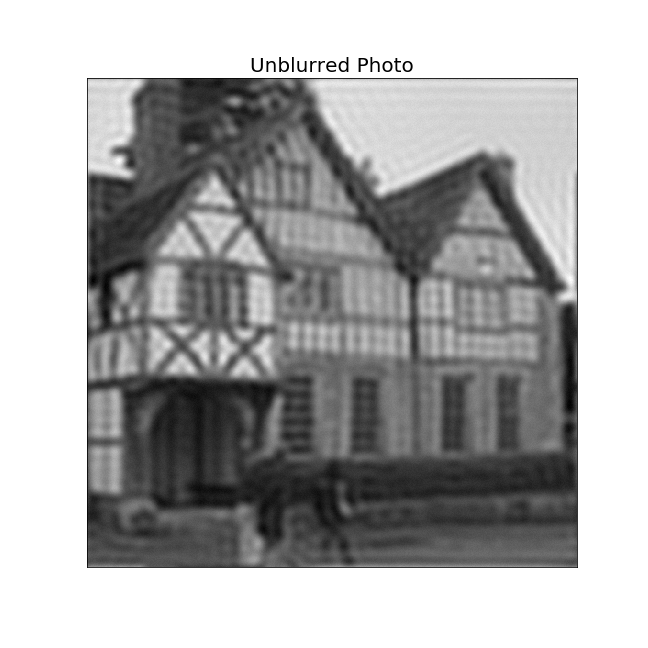
\includegraphics[width = 100mm]{unblurred.png}
\caption{The unblurred photo of \textquotedblleft blur.txt\textquotedblright with the point spread function Eq. \ref{eq:psf} and modified deconvolution function Eq. \ref{eq:dec}.}
\label{fig:unblur}
\end{figure}

\subsection*{d)}
The unblurred photo is apparently much sharper than the blurred, but there are still some wave-like shadows in the unblurred photo. This imperfection may come from our approximation when $\tilde{f}_k\to0$, to avoid overflow of $\tilde{a}_k$ and roundoff error. To see the effect of the error when $\tilde{f}_k\to0$, if $\epsilon=0$, i.e. there is no modification of the deconvolution function, then it returns an error due to overflow. Then if $\epsilon=10^{-5}$, for instance, the unblurred photo is plotted as Figure. \ref{fig:badunblur} shows. 

\begin{figure}[ht]
\centering
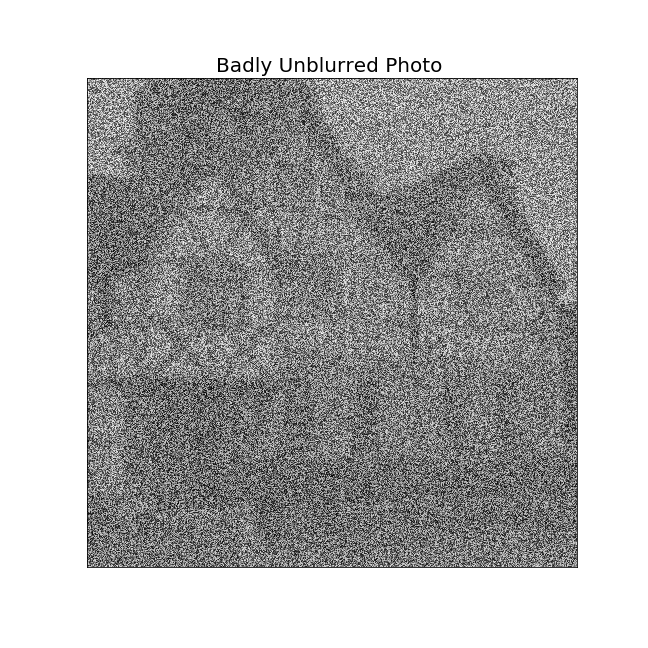
\includegraphics[width = 100mm]{bad_unblurred.png}
\caption{The unblurred photo of \textquotedblleft blur.txt\textquotedblright with the point spread function Eq. \ref{eq:psf} and modified deconvolution function Eq. \ref{eq:dec}, with $\epsilon=10^{-5}$.}
\label{fig:badunblur}
\end{figure}

The noises in Figure. \ref{fig:badunblur} is too serious that it nearly overshadows the correct picture. Let's have another try for a $\epsilon=10^{-4}$, the result of which is given in Figure. \ref{fig:bad4}. The result for $\epsilon=10^{-4}$ is much better in that the noise is more bearable and the wave-like errors is even slighter than Figure. \ref{fig:unblur}, seen in the sky. This means for $\epsilon<10^{-3}$, the roundoff error grows faster as $\tilde{f}_k$ goes smaller. So even though a smaller $\epsilon$ may allow a sharper photo, to avoid strong noise, $10^{-3}$ is about a smallest optimal value for it. 

\begin{figure}[ht]
\centering
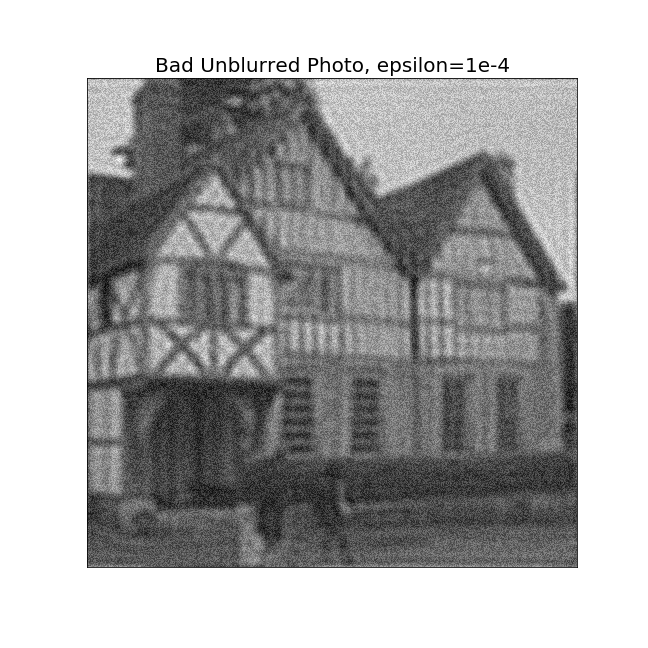
\includegraphics[width = 100mm]{bad_unblurred(1).png}
\caption{The unblurred photo of \textquotedblleft blur.txt\textquotedblright with the point spread function Eq. \ref{eq:psf} and modified deconvolution function Eq. \ref{eq:dec}, with $\epsilon=10^{-4}$.}
\label{fig:bad4}
\end{figure}

For some more practical problems, when the point spread function cannot be known exactly, there will be another part of error for the estimate of the point spread function, which also limits our ability to deblur a photo.


\end{document}